%%%%%%%%%%%%%%%%%%%%%%%%%%%%%%%%%%%%%%%%%%%%%%%%%%%%%%%%%%%%%%%%%%%%%%%%%%%%%%%%
%2345678901234567890123456789012345678901234567890123456789012345678901234567890
%        1         2         3         4         5         6         7         8

\documentclass[letterpaper, 10 pt, conference]{ieeeconf}  % Comment this line out
                                                          % if you need a4paper
%\documentclass[a4paper, 10pt, conference]{ieeeconf}      % Use this line for a4
                                                          % paper

\IEEEoverridecommandlockouts                              % This command is only
                                                          % needed if you want to
                                                          % use the \thanks command
\overrideIEEEmargins
% See the \addtolength command later in the file to balance the column lengths
% on the last page of the document



% The following packages can be found on http:\\www.ctan.org
%\usepackage{graphics} % for pdf, bitmapped graphics files
%\usepackage{epsfig} % for postscript graphics files
%\usepackage{mathptmx} % assumes new font selection scheme installed
%\usepackage{times} % assumes new font selection scheme installed
%\usepackage{amsmath} % assumes amsmath package installed
%\usepackage{amssymb}  % assumes amsmath package installed


\usepackage{graphicx}

\title{\LARGE \bf
Mobile Development of Philippine Climate Outlook Through Data Driven Documents and Web-View Applications
}

\author{Adrienne Elise R Cortez}

\begin{document}

\maketitle
\thispagestyle{empty}
\pagestyle{empty}


%%%%%%%%%%%%%%%%%%%%%%%%%%%%%%%%%%%%%%%%%%%%%%%%%%%%%%%%%%%%%%%%%%%%%%%%%%%%%%%%
\begin{abstract}

Knowing the amount of rainfall in a region is a necessity for people
to know if they need to plant crops or to evacuate areas based in the
heaviness of precipitation. The purpose of this project is to provide a
solution to easy access of the data that is already provided by
government agencies and to discuss how the development and the use of
a mobile app designed to carry the information from the SARAi website.
The technology used in this application is PhoneGap, which is a mobile
web-view application that allows the programmer to use familiar scripts
in coding within mobile applications and allows for a high percentage of
code reuse when coding for both web and mobile applications. In joint
with this technology, Data Driven Documents or D3 is used to display the
maps dynamically with the data supplied and less processing time than
what Geographical Information Systems provide

\end{abstract}


%%%%%%%%%%%%%%%%%%%%%%%%%%%%%%%%%%%%%%%%%%%%%%%%%%%%%%%%%%%%%%%%%%%%%%%%%%%%%%%%
\section{Introduction}

The vast land wealth and the tropical climate of the Philippines mean that our country has a lot of land for farming but is also very prone to natural disasters like typhoons. Many citizens have the need to know forecasts about factors of climate including average temperature and amount of rainfall in an area for their own safety and use. These pieces of information can also be presented in a different way so that farmers would be able to ascertain the type of crop they would need to plant in a certain timeframe or when to plant a certain type of crop. This leads to the need to have easy access to the information provided. According to recent studies, it says that the average Filipino has access to at least one device that is capable of connecting to the internet. With the spread of phones built from open source casual desktop users have migrated to using their portable handheld equivalent: smartphones. \setlength{\parskip}{6pt}

Several countries have websites that show climate outlook in varying degrees and varying ways. For example, National Weather Service of the US, Meteorological Agency of Japan and Hydrometcenter of Russia has a page on their website dedicated to displaying this information. The Philippines’ PAG-ASA has a website that show these data in the form of colored maps but these are not easily accessible when not connected to the internet. The mobile application will be largely offline, and will only need to connect to the internet every time information is updated.

\section{Review of Related Literature}

Visualization of Data is a great way for people to be able to know how their data works without having to do much of an effort regarding it. Rows upon rows and columns upon columns of data and information can be stored easily in a spreadsheet but these data are not easy to understand without the help of some tools or a lot of skill with regards to the given information. For example, when you see the rise and fall of the values in the stock market for example, numbers could be dizzying in large amounts, and people have long since proven to understand and retain illustrations and visual cues better than other types of sensory input. \cite{TurnerUX} Current technologies used in the display of location-oriented datasets, for example rainfall forecasts, are of the following: a) using Geographical Information Systems (GIS) available to the public, for example Google Maps or Apple Maps. However, previous systems using GIS for these factors are limited due to the processing speed and the amount of data that GIS uses to display what is needed, therefore, a more basic visualization is needed for a more convenient use of the provided data.\setlength{\parskip}{6pt}

Geographical Information Systems work in a variety of levels, and is used to power many different decisions that might affect a lot of people. GIS, put into simple terms, does four major things: 1)  it creates geographical data, 2) manages geographical data, 3) analyzes these data and 4) displays it in the form of a map. Several different types of people contribute to make a GIS work, and that includes cartographers, land surveyors, analysts, programmers. Although GIS are incredibly useful for making these decisions, many GIS are already loaded with a lot of information about a lot of things across the globe and not specifically focused locally.\cite{gis} This has good effects and bad effects to the visualization of data. A large quantity of data means that the length of time needed for the information to be loaded is longer but in this certain scenario where we only focus on the forecast per municipality per province in the Philippines, such amount of detail is not needed. \setlength{\parskip}{6pt}

This is where SVG, D3JS and GeoJSON come in. D3JS stands for Data Driven Documents JavaScript. D3JS is a JavaScript Framework that was made for the display of and/or visualization of objects given a certain amount of data. Given that it is an open source JavaScript framework, simply sourcing the D3JS file would be all the preparation needed for your coding environment.\setlength{\parskip}{6pt}

JSON behave similarly to objects in JavaScript and GeoJSON files are a subset of JSON.\cite{JSONatWork} GeoJSON are relatively small files which have details about certain regions or provinces that would be useful in illustrating these said regions. There are different open source GeoJSON files in GitHub and other project platforms and could be used in a project without further need to use other resources. GeoJSON files have ‘features’ and some of these features may include the name of the certain region or the country or the geographic parent of the certain region but the most important part of the GeoJSON files is its geometry. The geometry of an object in a GeoJSON file has two important properties: 1) the type and 2) the coordinates. The type of the GeoJSON object is a structure that lets you know how the coordinates would be laid out or how much information you would be able to put in the coordinates. For example, a Point would only need two coordinates in the form of a Point while a LineString would need you to have an array of points. What we use in mapping geographical borders are the type MultiPolygon. A MultiPolygon is an array of array of array of Points. These points construct the region according to the coordinates of the widely-used Geographic Coordinate System (latitude and longitude), also called the e that you see in regular maps. The Philippines for example sits ~13 degrees North of the Equator and ~122 degrees East of the Prime Meridian. \cite{geojson} \setlength{\parskip}{6pt}


\begin{figure}[h!]
\centering
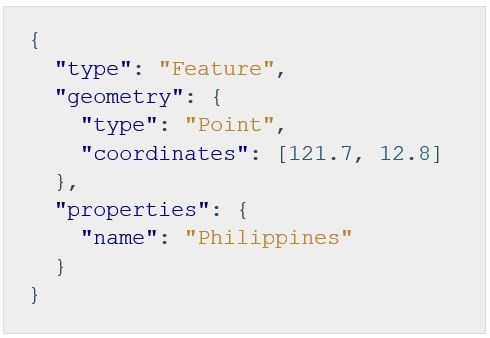
\includegraphics[scale=.6]{point.jpg}
\caption{An Example of a GeoJSON object, type: Point}
\label{fig:point}
\end{figure}

\section{Methodology}

The technology used in this application is PhoneGap, which is a mobile web-view application that allows the programmer to use familiar scripts in coding within mobile applications and allows for a high percentage of code reuse when coding for both web and mobile applications.\setlength{\parskip}{6pt}

The user interface is made by the HTML skeleton and local CSS and the system functionalities use JavaScript. The initial data is loaded via a CSV file. The format of the csv file is as follows: 1) The first row is the headers where the title of the first column doesn’t matter but the headers of the values of each month must be in text format  (can be achieved by pressing ctrl+1 for the selected cells using Excel as Excel automatically converts any type of date inputted into cells into a date format), and preferably contain both the month and the year of the values for each column; 2) the contents of each of the rows must start with the name of the province followed by each of its municipalities. 

\begin{figure}[h!]
\centering
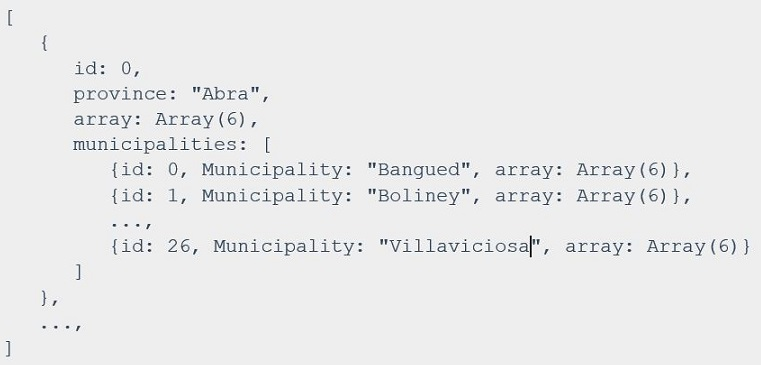
\includegraphics[scale=.5]{object}
\caption{Object Storage of Parsed Data}
\label{fig:object}
\end{figure}

The data from the csv file is parsed using a preset list of the names of all the provinces of the Philippines and is stored in an array of objects which we will call provinceArray in this document as shown in Figure 1 where “Array(6)” contains the values of each month for each municipality/province given by the csv file. Headers of the csv file are put aside to a smaller array to avoid repetition in the already large object provided by the parsing.\setlength{\parskip}{6pt}

After the files are parsed, the maps are created using D3JS and GeoJSON files. The GeoJSON file for the Philippine provinces is downloaded from GitHub and is used as the path attribute of the <svg> tag. The colors of each province are taken from the provinceArray object presented in Figure 1 with the corresponding nth map to the nth element of the array for each province. The color scheme is selected by the user upon the first startup of the app, and is given four ranges according to number of millimeters of rainfall in that region. The ranging is applied to the corresponding value and then is assigned as the color of that province of that month. Six maps are crafted by D3JS in SVG and the headers of the previous columns of the csv file are put as a label of each map. Consequently, the initial display of the app selects the first province in the list to show the summary of the rainfall for that province for the next six months by selecting the 0th element of the provinceArray object and rounding the two-decimal number to a round natural number. Each display box shows that month/year, the rain in mm and is colored according to the selected scheme. \setlength{\parskip}{6pt}

Two-way binding is used to display the tabulated form of the data with their respective coloring based on ranges.

\begin{figure}[h!]
\centering
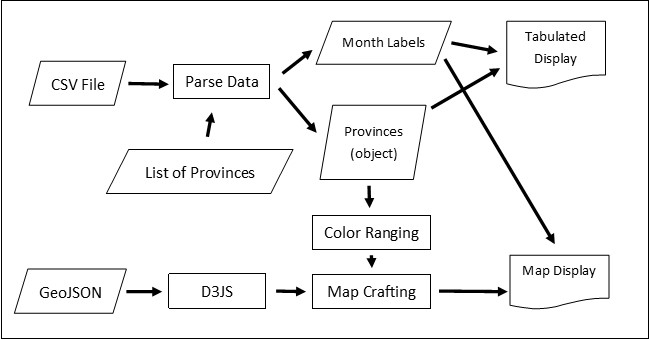
\includegraphics[scale=.5]{development}
\caption{Flow Chart Summary of Methodology}
\label{fig:development}
\end{figure}

\section{Results and Discussion}

The app starts up with none of its settings and data setup. The processing is front-loaded, so the app, once it is fully loaded no longer needs to add any middle processes that slow down the use of the app. Initial loading of the data takes around 40 seconds to 45 seconds, averaging to below a minute at 43 seconds. This loading only takes place the first time that the user opens the app, or after an application update has been downloaded. The loaded data is stored inside the phone’s internal storage, provided that the user allows the app to access files. This lessens the processing time that the app needs for its startup. \setlength{\parskip}{6pt}


\begin{figure}[h!]
\centering
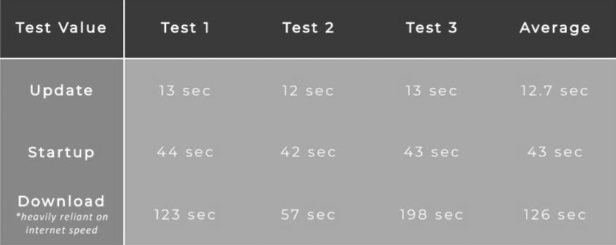
\includegraphics[scale=.5]{table}
\caption{Usage Time-Consumption Table}
\label{fig:table}
\end{figure}

The home page consists of dropdowns of all provinces and municipalities, and once selected, the displayed details will correspond to the selected province/municipality. It also shows the Six Month Nationwide Rainfall Outlook that shows the amount of rainfall in a province by color ranging the provinces in shades of blue.\setlength{\parskip}{6pt}

Updating the information of the app is done by updating the app itself. Since the available information for rainfall in an area spans 6-months, the data of the app changes monthly. This can be done by downloading the current version of the app either through Google Play Store (once available) or the QR code.


\begin{figure}[h!]
\centering
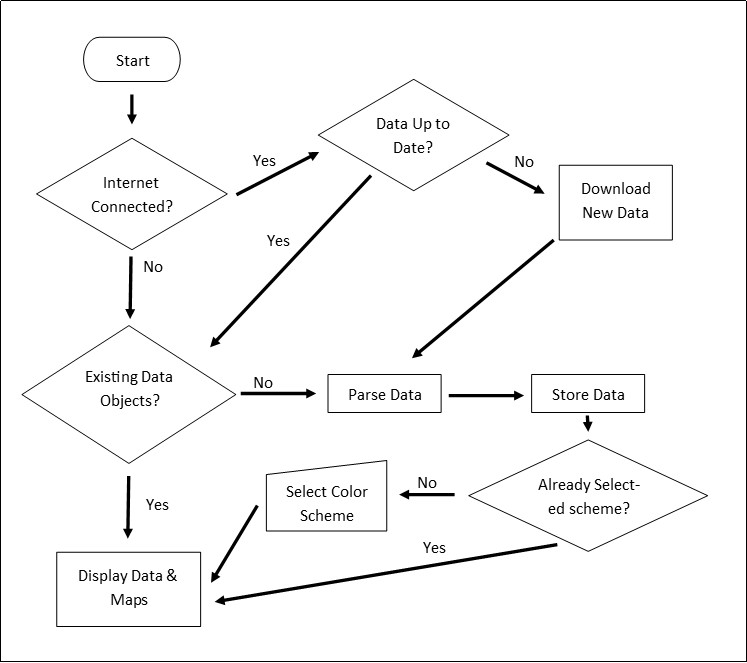
\includegraphics[scale=.4]{usecases}
\caption{Flow Chart Summary of Use Cases}
\label{fig:usecases}
\end{figure}

\section{CONCLUSIONS}

The Rainfall Outlook Application for the Philippines was successfully created to display the rainfall in an province or municipality with the stipulation of simplicity and lesser strain on the computational device. The application performs better when many of the components have been preloaded or stored into a data object that can be re-accessed at a later date. \setlength{\parskip}{6pt}

Visualization of Data helps make decisions for those that need there information because people recognize and recall visual cues better than other sensory input.

\addtolength{\textheight}{-12cm}   % This command serves to balance the column lengths
                                  % on the last page of the document manually. It shortens
                                  % the textheight of the last page by a suitable amount.
                                  % This command does not take effect until the next page
                                  % so it should come on the page before the last. Make
                                  % sure that you do not shorten the textheight too much.

%%%%%%%%%%%%%%%%%%%%%%%%%%%%%%%%%%%%%%%%%%%%%%%%%%%%%%%%%%%%%%%%%%%%%%%%%%%%%%%%



%%%%%%%%%%%%%%%%%%%%%%%%%%%%%%%%%%%%%%%%%%%%%%%%%%%%%%%%%%%%%%%%%%%%%%%%%%%%%%%%


\bibliography{reference} 
\bibliographystyle{plain}


\end{document}
